%Plan et documentation de déploiement

%déploiement sur appbase.io

Le déploiment de l'application se passe en trois étapes.
Premièrement, les documents a traiter (au format pdf) doivent être placés dans un dossier, ou ils seront récupérés un par un par un script qui en extrayera la texte brut, qui sera lui même analysé pour en tirer les données.
Ces données seront alors ajouter à un fichier JSON dont le format correspond à ce que Reactivesearch attend.
Puis le JSON ainsi crée doit être ajouté dans notre moteur de recherche.

\subsection{Récupération du transcript d'un document}
La chaine de traitement commence par l'extraction du texte des documents pdf.
Pour cela, le script `extractText.sh' va tester tous les documents selon la méthode suivante:\newline
Utilisation de pdftotext: Si du texte peut être extrait du pdf courant, ce texte est stocké dans un nouveau fichier et le script passe au document suivant.\newline
Si aucun texte n'a pu être extrait, le script charge Tesseract (OCR) en mémoire, découpe le document en pages qui sont individuellement passées par un script de traitement d'image.
Les images traitées individuellement sont alors rassemblées dans un fichier au format tiff, transmis a Tesseract qui se charge d'en extraire le texte.

L'extraction dure environ 1h10 pour nos 431 fichiers.

Quand l'exécution de ce script est terminée, on obtient un dossier contenant les transcripts de chaque fichiers traités en format txt.

\subsection{Extraction des données}
L'utilisation du script python `reactiv\_json.py' permet de créer un fichier au format JSON pouvant être lu par Reactivesearch.
Ce script commence par lire chaque fichier de transcript au format txt crées précédemment et en extraire les informations avec les bibliothèques python situées dans le dossier `utils'.

L'extraction de toutes les données pour le format JSON dure environ 40 minutes pour nos 431 documents.

Le fichier crée par ce script est directement utilisable avec le moteur de recherche.

\subsection{Moteur de recherche}
%Le moteur de recherche fonctionne comme machin machin machin
Le moteur de recherche basé sur ElasticSearch et Reactivesearch est utilisable tel quel au lien suivant: \href{https://ujcqr.csb.app}{Moteur de recherche}.
Il est directement disponible en ligne et ne nécessite pas de nouvelle installation.

Cependant le moteur de recherche n'est pas interactif: aucune action n'est directement possible sur les données.
Pour modifier, ajouter, retirer des données au site internet, il faut directement passer par l'application Appbase.io ou le JSON contenant nos données sont stockées.

L'import/modification/suppression des données peut y être réaliser en ligne.
L'import d'un nouveau JSON est également possible si le format du JSON respecte certaines normes. 
La structure du JSON est la suivante:

\begin{figure}[h!]
  \centering
	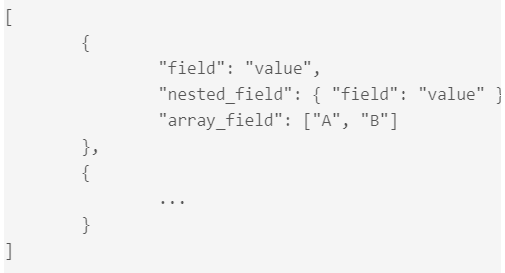
\includegraphics[width=0.5\textwidth]{FormatJsonAppbase.PNG}
	\caption[]{Exemple de format accepté sous Appbase}
	\label{}
\end{figure}

Lorsque les données sont correctement importées, un mail contenant l'identifiant du JSON (credentials) afin de sécuriser l'utilisation des données. 

Cette méthode n'est pas très ergonomique mais l'ergonomie de cette partie n'est pas nécessaire pour ce POC\@.
